% Created by tikzDevice version 0.12.3.1 on 2021-01-15 14:26:40
% !TEX encoding = UTF-8 Unicode
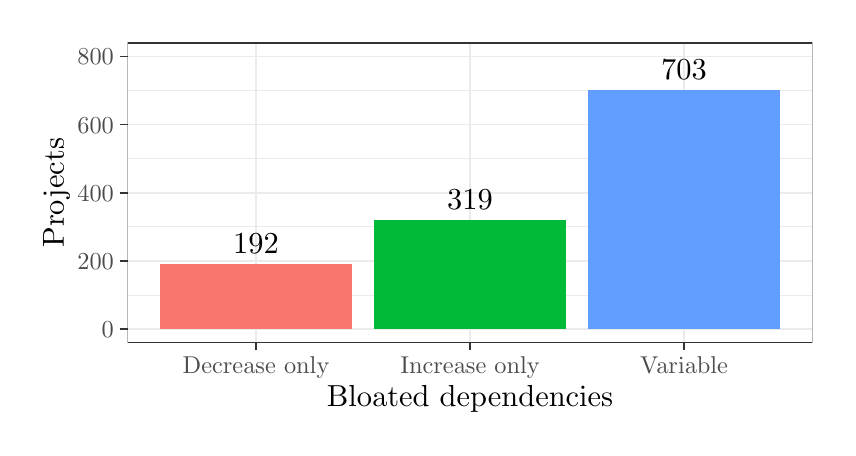
\begin{tikzpicture}[x=1pt,y=1pt]
\definecolor{fillColor}{RGB}{255,255,255}
\path[use as bounding box,fill=fillColor,fill opacity=0.00] (0,0) rectangle (289.08,144.54);
\begin{scope}
\path[clip] (  0.00,  0.00) rectangle (289.08,144.54);
\definecolor{drawColor}{RGB}{255,255,255}
\definecolor{fillColor}{RGB}{255,255,255}

\path[draw=drawColor,line width= 0.6pt,line join=round,line cap=round,fill=fillColor] (  0.00,  0.00) rectangle (289.08,144.54);
\end{scope}
\begin{scope}
\path[clip] ( 36.11, 30.69) rectangle (283.58,139.04);
\definecolor{fillColor}{RGB}{255,255,255}

\path[fill=fillColor] ( 36.11, 30.69) rectangle (283.58,139.04);
\definecolor{drawColor}{gray}{0.92}

\path[draw=drawColor,line width= 0.3pt,line join=round] ( 36.11, 47.92) --
	(283.58, 47.92);

\path[draw=drawColor,line width= 0.3pt,line join=round] ( 36.11, 72.55) --
	(283.58, 72.55);

\path[draw=drawColor,line width= 0.3pt,line join=round] ( 36.11, 97.18) --
	(283.58, 97.18);

\path[draw=drawColor,line width= 0.3pt,line join=round] ( 36.11,121.80) --
	(283.58,121.80);

\path[draw=drawColor,line width= 0.6pt,line join=round] ( 36.11, 35.61) --
	(283.58, 35.61);

\path[draw=drawColor,line width= 0.6pt,line join=round] ( 36.11, 60.24) --
	(283.58, 60.24);

\path[draw=drawColor,line width= 0.6pt,line join=round] ( 36.11, 84.86) --
	(283.58, 84.86);

\path[draw=drawColor,line width= 0.6pt,line join=round] ( 36.11,109.49) --
	(283.58,109.49);

\path[draw=drawColor,line width= 0.6pt,line join=round] ( 36.11,134.11) --
	(283.58,134.11);

\path[draw=drawColor,line width= 0.6pt,line join=round] ( 82.51, 30.69) --
	( 82.51,139.04);

\path[draw=drawColor,line width= 0.6pt,line join=round] (159.85, 30.69) --
	(159.85,139.04);

\path[draw=drawColor,line width= 0.6pt,line join=round] (237.18, 30.69) --
	(237.18,139.04);
\definecolor{fillColor}{RGB}{0,186,56}

\path[fill=fillColor] (125.05, 35.61) rectangle (194.65, 74.89);
\definecolor{fillColor}{RGB}{248,118,109}

\path[fill=fillColor] ( 47.71, 35.61) rectangle (117.31, 59.25);
\definecolor{fillColor}{RGB}{97,156,255}

\path[fill=fillColor] (202.38, 35.61) rectangle (271.98,122.17);
\definecolor{drawColor}{RGB}{0,0,0}

\node[text=drawColor,anchor=base,inner sep=0pt, outer sep=0pt, scale=  1.10] at (159.85, 78.69) {319};

\node[text=drawColor,anchor=base,inner sep=0pt, outer sep=0pt, scale=  1.10] at ( 82.51, 63.05) {192};

\node[text=drawColor,anchor=base,inner sep=0pt, outer sep=0pt, scale=  1.10] at (237.18,125.97) {703};
\definecolor{drawColor}{gray}{0.20}

\path[draw=drawColor,line width= 0.6pt,line join=round,line cap=round] ( 36.11, 30.69) rectangle (283.58,139.04);
\end{scope}
\begin{scope}
\path[clip] (  0.00,  0.00) rectangle (289.08,144.54);
\definecolor{drawColor}{gray}{0.30}

\node[text=drawColor,anchor=base east,inner sep=0pt, outer sep=0pt, scale=  0.88] at ( 31.16, 32.58) {0};

\node[text=drawColor,anchor=base east,inner sep=0pt, outer sep=0pt, scale=  0.88] at ( 31.16, 57.21) {200};

\node[text=drawColor,anchor=base east,inner sep=0pt, outer sep=0pt, scale=  0.88] at ( 31.16, 81.83) {400};

\node[text=drawColor,anchor=base east,inner sep=0pt, outer sep=0pt, scale=  0.88] at ( 31.16,106.46) {600};

\node[text=drawColor,anchor=base east,inner sep=0pt, outer sep=0pt, scale=  0.88] at ( 31.16,131.08) {800};
\end{scope}
\begin{scope}
\path[clip] (  0.00,  0.00) rectangle (289.08,144.54);
\definecolor{drawColor}{gray}{0.20}

\path[draw=drawColor,line width= 0.6pt,line join=round] ( 33.36, 35.61) --
	( 36.11, 35.61);

\path[draw=drawColor,line width= 0.6pt,line join=round] ( 33.36, 60.24) --
	( 36.11, 60.24);

\path[draw=drawColor,line width= 0.6pt,line join=round] ( 33.36, 84.86) --
	( 36.11, 84.86);

\path[draw=drawColor,line width= 0.6pt,line join=round] ( 33.36,109.49) --
	( 36.11,109.49);

\path[draw=drawColor,line width= 0.6pt,line join=round] ( 33.36,134.11) --
	( 36.11,134.11);
\end{scope}
\begin{scope}
\path[clip] (  0.00,  0.00) rectangle (289.08,144.54);
\definecolor{drawColor}{gray}{0.20}

\path[draw=drawColor,line width= 0.6pt,line join=round] ( 82.51, 27.94) --
	( 82.51, 30.69);

\path[draw=drawColor,line width= 0.6pt,line join=round] (159.85, 27.94) --
	(159.85, 30.69);

\path[draw=drawColor,line width= 0.6pt,line join=round] (237.18, 27.94) --
	(237.18, 30.69);
\end{scope}
\begin{scope}
\path[clip] (  0.00,  0.00) rectangle (289.08,144.54);
\definecolor{drawColor}{gray}{0.30}

\node[text=drawColor,anchor=base,inner sep=0pt, outer sep=0pt, scale=  0.88] at ( 82.51, 19.68) {Decrease only};

\node[text=drawColor,anchor=base,inner sep=0pt, outer sep=0pt, scale=  0.88] at (159.85, 19.68) {Increase only};

\node[text=drawColor,anchor=base,inner sep=0pt, outer sep=0pt, scale=  0.88] at (237.18, 19.68) {Variable};
\end{scope}
\begin{scope}
\path[clip] (  0.00,  0.00) rectangle (289.08,144.54);
\definecolor{drawColor}{RGB}{0,0,0}

\node[text=drawColor,anchor=base,inner sep=0pt, outer sep=0pt, scale=  1.10] at (159.85,  7.64) {Bloated dependencies};
\end{scope}
\begin{scope}
\path[clip] (  0.00,  0.00) rectangle (289.08,144.54);
\definecolor{drawColor}{RGB}{0,0,0}

\node[text=drawColor,rotate= 90.00,anchor=base,inner sep=0pt, outer sep=0pt, scale=  1.10] at ( 13.08, 84.86) {Projects};
\end{scope}
\end{tikzpicture}
